\documentclass[12pt, a4paper]{article}
\usepackage[english]{babel}
\usepackage{graphicx}
\usepackage[hyphens]{url}
\usepackage{fullpage}
\usepackage{amsmath}
\usepackage[colorinlistoftodos]{todonotes}
\usepackage{subcaption}
\usepackage{setspace} 
%\doublespacing


\begin{document}
\title{\sc Opioid Deaths by Race in the \\ United States, 2000--2015}
\author{Monica Alexander\footnote{\texttt{monicaalexander@berkeley.edu}} \\ \emph{University of California, Berkeley}  \and Magali Barbieri\footnote{\texttt{magali@demog.berkeley.edu}} \\ \emph{University of California, Berkeley} and \\\emph{Institut national d'\'{e}tudes d'\'{e}mographiques} \and Mathew Kiang\footnote{\texttt{mkiang@mail.harvard.edu}} \\ \emph{Harvard T.H.\ Chan School of Public Health}}
\date{Paper presented at PAA 2017 \\ Session 133: Trends and Causes of Adult Mortality in the United States}

\maketitle

\begin{abstract}
The opioid-related mortality rate in the United States more than tripled between 2000 and 2015. However, there were stark differences in the trend for the non-Hispanic black and non-Hispanic white populations. In this paper we assess differences in opioid deaths by race. We analyze patterns and trends in multiple cause-of-death data to gain a better understanding of how deaths differ by race and what has contributed to changes over time. The trend in race-specific opioid death rates over 2000--2015 can be divided into two periods: 2000--2010 and 2010--2015. The increase in 2000--2010 was more substantial for the white population and was driven by prescription painkillers. Since 2010, the rates of opioid-mortality increase for both the white and black populations have been similar and largely due to heroin and fentanyl-type opioids. For the white population, death rates due to heroin and fentanyl-type drugs decrease with age, but for the black population, the opposite is true. In addition, the number of deaths that involve more than one opioid drug has increased over time, with the rate of increase coinciding with the overall rate of increase in opioid deaths. 
\end{abstract}

\setlength\parindent{0pt} 
\setlength{\parskip}{\baselineskip}% 

%%%%%%%%%%%%%%%%%%%%%%
\section{Introduction}
The number of opioid-related deaths in the United States has increased since 2000 and that increase has accelerated since 2010 (Figure \ref{fig:nood}). This is unique among deaths due to drugs as the rate of non-opioid drug deaths has been relatively constant since 2005. In 2015 there were around 33,200 deaths due to opioid-related overdoses. This corresponds to a death rate of 10 per 100,000 people in 2015, which has more than tripled from 3 per 100,000 people in 2000. 
\begin{figure}[h!]
 \centering
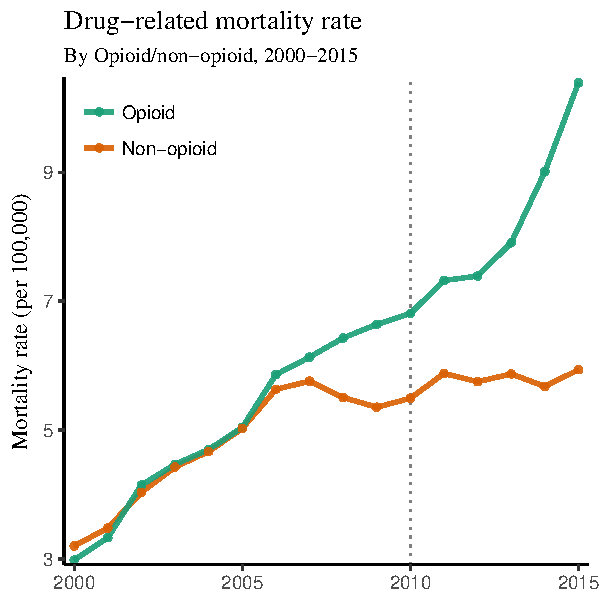
\includegraphics[width=0.5\textwidth]{./plots/paper_fig1_nood_v.pdf} 
 \caption{Opioid and non-opioid related drug overdoses, 2000--2015}
 \label{fig:nood}
\end{figure}

The substantial increase in opioid deaths has drawn national attention and become an important part of the political agenda. The Obama administration introduced initiatives to expand addiction treatment and increase coverage for mental health and substance abuse services. President Obama also asked Congress to pass \$1.1 billion in new funding to increase the availability of treatment for opioid use disorders (White House, 2016). The opioid epidemic is also a focus of the new administration. In March 2017, President Trump signed an executive order to create a national opioid commission (White House, 2017). The commission is to: examine the funding aimed at reducing addiction rates; assess the availability of treatment services; and review the effectiveness of state prescription drug monitoring programs. 

Death rates due to opioids are higher in the non-Hispanic white population compared with the non-Hispanic black population (Figure \ref{fig:overall}).\footnote{Throughout this paper, we refer to the non-Hispanic white population and non-Hispanic black population as the white population and black population, respectively.} While opioid deaths rates for the two populations were similar in 2000, by 2005 the death rate for the white population was 1.6 times that of the black population, with this ratio peaking at 2.4 in 2010. (Figure \ref{fig:overall_rr}). The latest data, from 2015, indicate the opioid death rate for the white population is around 12.5 deaths per 100,000 people, almost double that of the black population. Over the period 2010--2015, the death rate increased by 51 per cent for the white population and 87 per cent for the black population. 

The trend in race-specific opioid death rates over 2000--2015 can be divided into two periods: 2000--2010 and 2010--2015. Much of the mortality gap between the white and black population is due to patterns during the first period (2000--2010): white mortality rates increased while black mortality rates steadied. As such the relative risk between the two groups peaked in 2010. However, in the second period, the rates of increase in opioid deaths for both population groups have been similar, and the relative risk has declined. 

\begin{figure}[h!]
\begin{subfigure} [b]{0.5\textwidth} 
 \centering
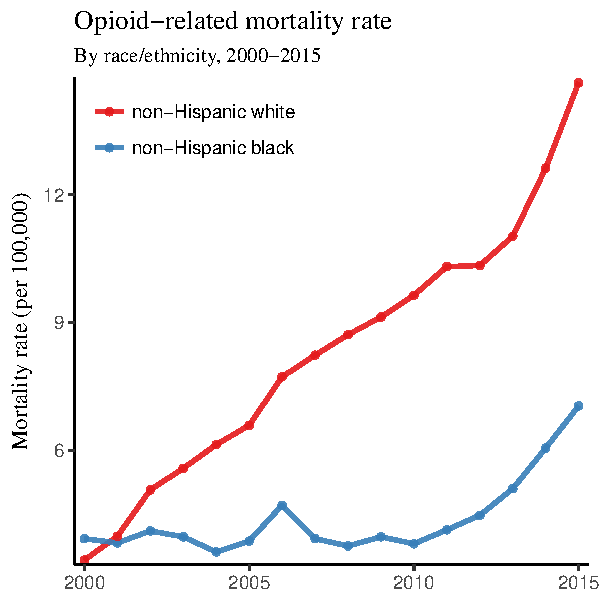
\includegraphics[width=0.95\textwidth]{./plots/paper_fig2_overall_adjusted.pdf} 
 \caption{Opioid-related mortality rate by race, 2000--2015}
 \label{fig:overall}
 \end{subfigure} ~
 \begin{subfigure} [b]{0.5\textwidth} 
 \centering
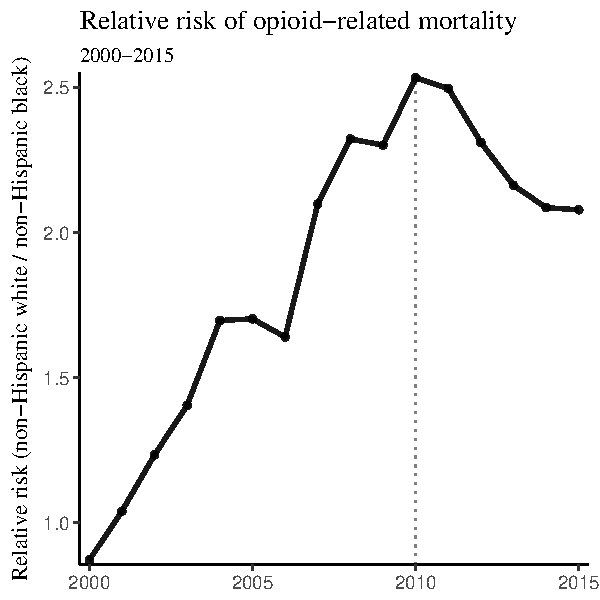
\includegraphics[width=0.95\textwidth]{./plots/paper_fig2_relative_risk_v.pdf} 
 \caption{Relative risk of opioid mortality by race, 2000--2015}
 \label{fig:overall_rr}
 \end{subfigure} ~
  \caption{Trends in opioid death by race 2000--2015.}
\end{figure}

The presence of higher opioid death rates for the white population has led to commentators referring to the opioid epidemic as `white only', focusing on trends in deaths for the white population (e.g.,\ Lane, 2016; Kolata \& Cohen, 2016). Indeed, the combination of high opioid death rates, as well as a lower overall death rate compared to the black population, means that the impact is more noticeable in the white population. For example, opioid drug overdoses comprise some of the `deaths of despair' (i.e.\ deaths due to drugs, alcohol and suicide) that Case and Deaton (2017) attributed to causing an increase in the mortality rate in the non-Hispanic white population aged 45-54. However, given that the shift in 2010 has caused opioid-related death rates in the black population to increase at much the same rate, it is an issue for both populations. The trend since 2010 in the black population is perhaps even more startling, given the experience in the earlier part of the century was so different and the cumulative effect from previously high rates is absent.

In this paper, we analyze patterns and trends in multiple cause-of-death data to gain a better understanding of opioid deaths, how they differ by race and what has contributed to the change in trends over time. We focus on two aspects. Firstly, we investigate age patterns in opioid deaths by race. Given that opioid-related deaths cover a wide range of prescriptions and illicit drugs, we expect large differences in deaths across the age dimension. Secondly, we utilize the multiple cause of-death data to explore trends in deaths due to a combination of drugs and underlying causes. While previous research has highlighted the substantial increase in opioid deaths, especially for the younger white population (e.g.,\ Paulozzi et al.\ 2006; Dart et al.\ 2015; Frenk et al.\ 2015; and Rudd et al.\ 2016), we offer a comparison of opioid deaths stratified by race and age, and consider trends due to drug combinations. 

We observe that the increase in both populations has been largely due to accidental overdoses due to opioids or a mixture of opioids and other drugs. The increase in 2000--2010 was more substantial for the white population and was driven by prescription painkillers. Since 2010, the rates of opioid-mortality increase for both the white and black populations have largely been due to heroin and synthetic opioids other than methadone (mostly fentanyl). Age patterns in opioids show an inverted pattern by race, with mortality due to heroin and fentanyl-type drugs decreasing with age in the white population, but increasing with age for the black population. The number of deaths involving more than one opioid drug has increased over time for both races, with the rate of increase coinciding with the overall rate of increase in opioid deaths. Our descriptive analysis is a starting point for future research using other datasets and more sophisticated demographic and statistical techniques.

The remainder of the paper is structured as follows. In the next section we describe the data and how opioid deaths were defined. Section \ref{section:overall} then describes trends in race-specific opioid death rates by underlying cause of death and opioid drug. In Section \ref{section:age} we analyze age-specific mortality rates by race and type of opioid drug. We then investigate trends in the presence of multiple opioids in an overdose in Section \ref{section:multiple_cause}. We conclude with a discussion of the main questions raised by the analysis, and directions for future work. 

%%%%%%%%%%%%%%%%%%%%%
\section{Data}
The analysis in this paper uses multiple cause-of-death mortality data available through the National Vital Statistics System of the National Center for Health Statistics (NCHS, 2000--2015). These data files provide multiple cause-of-death information for deaths occurring within the United States. Information on cause of death is extracted from death certificates filed in the vital statistics offices of each state and the District of Columbia. We restrict our analysis to consider the non-Hispanic white and non-Hispanic black population. Throughout the paper, all overall mortality rates have been age-standardized using 10-year age groups (0-9, 10-19, \dots, 80+) and the 2000 Census population as a standard. 

We restrict our analysis to the period 2000--2015. During this period, causes of death were coded according to the International Classification of Diseases, Tenth Revision (ICD-10) (WHO 2016). There were minimal changes to ICD-10 over the fifteen years that would affect the trends in causes-of-death related to opioids. However, there were two updates to coding rules that may have small impacts (WHO 2017). The first, in 2002, was to give preference to acute poisoning over substance-abuse syndromes. If these are both indicated on a death certificate, acute poisoning should be selected as the underlying cause of death. Secondly, the 2006 update saw the introduction of a priority list for substances involved in drug poisonings, which prioritized opioids over other substances. 

\subsection{Defining deaths due to opioids}
We define deaths due to opioids in three ways. The first, is opioid drug overdose deaths, which makes up many opioid deaths. These are defined to have any combination of an underlying cause of death code and drug poisoning code (`T-code') listed in the table below (Table \ref{overdose-codes}). Codes in the left column refer to poisoning by, and exposure to, noxious substances, with different intents: accidental or unintended overdose (X40s); suicide or intended overdose (X60s); homicide (X85); or undetermined intent (Y10s). In practice, the determination of suicide can be difficult, and requires sufficient evidence of self-inflicted harm and intention to self-harm (Davis et al.\ 2013). In addition, the National Association of Medical Examiners recommend that `undetermined' intent be reserved for ``\dots the rare cases in which evidence exists to support more than one possible determination, that is, where some evidence suggests accident and other evidence suggests suicide or homicide.'' (Davis et al.\ 2013, p. 104). In practice, these criteria lead to accidental deaths being the most common intent underlying opioid overdose deaths. 

Within each underlying cause code group, the different numbers refer to different types of drugs. In particular, X42, X62 and Y12 refer to poisoning by (and exposure to) narcotics and psychodysleptics, which includes opioids, cocaine, LSD and cannabis. However, opioid T-codes can also appear in deaths by other noxious substances if multiple drugs are present. For example, X44 refers to accidental poisoning by (and exposure to) other and unspecified drugs. 

The T-codes cluster opioids into six main groups. `Other natural' and semi-synthetic opioids (T402), including codeine, morphine, hydrocodone and oxycodone. `Other synthetic' opioids includes drugs such as tramadol, fentanyl and fentanyl derivatives such as acetyl-fentanyl and furanyl-fentanyl. %While pharmaceutical fentanyl is a synthetic opioid pain reliever, there is an increasing presence of illegally-made fentanyl in the United States (CDC 2016). It can be mixed with heroin to increase its effect.

\begin{table}[h!]
\centering
\caption{Defining opioid-related overdose deaths}

\begin{tabular}{ll|ll}
\multicolumn{2}{l|}{Underlying cause} & \multicolumn{2}{l}{Associated drug poisoning cause} \\ \hline
Codes      & Meaning                 & Code               & Drugs                           \\ \hline
X40-44     & Unintended overdose     & T400               & Opium                           \\
X60-64     & Suicide                 & T401               & Heroin                          \\
X85        & Homicide                & T402               & Other natural                   \\
Y10-14     & Intent undetermined     & T403               & Methadone                       \\
           &                         & T404               & Other synthetic                 \\
           &                         & T406               & Unspecified opioid             
\end{tabular}
\label{overdose-codes}
\end{table}

In addition to opioid-related drug overdoses, we consider deaths with an underlying cause of death listed as F110--F119. The F11 family refers to mental and behavioral disorders due to opioid use. The third number refers to the type of disorder. For example, F111 refers to `harmful use', defined as ``(a) pattern of psychoactive substance use that is causing damage to health. The damage may be physical (as in cases of hepatitis from the self-administration of injected psychoactive substances) or mental (e.g.\ episodes of depressive disorder secondary to heavy consumption of alcohol)'' (WHO 2016).

Finally, we also consider deaths with any underlying cause that lists one of the opioid T-codes as a contributing cause of death, even if a drug overdose was not the underlying reason. Although opioid-related drug overdoses account for most opioid-related deaths, we also want to track trends in other opioid-type deaths over time. 


%%%%%%%%%%%%%%%%%%%%%%%

\section{Trends in opioid death rates by cause and type} \label{section:overall}
\subsection{Opioid death rates by underlying cause}
We begin by decomposing the overall mortality rates in Figure \ref{fig:overall} according to underlying cause of death and opioid type. Figure \ref{fig:code_race} shows the mortality rate by the four main underlying cause of death codes and race over time. The four largest categories account for over 83 per cent of all opioid-related deaths in 2000 and over 91 per cent in 2015. The four largest categories for both races are X42 (accidental drug overdose due to narcotics and psychodysleptics, which includes opioids, cocaine, LSD and cannabis); X44 (accidental drug overdose due to unspecified drugs); Y12 (drug overdose due to narcotics and psychodysleptics with intent unclear); and X64 (suicide by drug overdose due to unspecified drugs). 

For both the white and black population, many deaths are due to accidental drug overdoses (codes X42 and X44). As mentioned, the X42 category specifically includes opioids as the cause of death, whereas the X44 category is used most commonly when the death was caused by a mixture of drugs, and the main cause of fatality is unclear. Therefore, these groups may imply different types of overdoses --- while deaths in the X42 may only involve one type of opioid, deaths in the X44 group have occurred from a mixture of drugs. 

While the rates for X42 and X44 have steadily increased for the white population, the increase in X42 for the black population has mostly occurred in the last five years. This is the cause of the overall trend observed in Figure \ref{fig:overall}. As seen in Figure \ref{fig:nood}, non-opioid drug overdoses have also increased, but the rate of increase has not been as large, and has leveled off in recent years. The earlier increase in X44 for the black population has been partially offset by a decrease in Y12, which is opioid-related overdoses of undetermined intent. Deaths of undetermined intent are higher for the black population, which may understate black deaths rates of accidents and suicides. However, the undetermined intent death rate has generally decreased over time.

The rate of opioid-related drug overdoses that are deemed intentional (suicides) is higher for the white population, and has steadily increased over time. The largest suicide category is X64, which implies taking a mixture of opioid and non-opioid drugs. 

\begin{figure}[h!]
 \centering
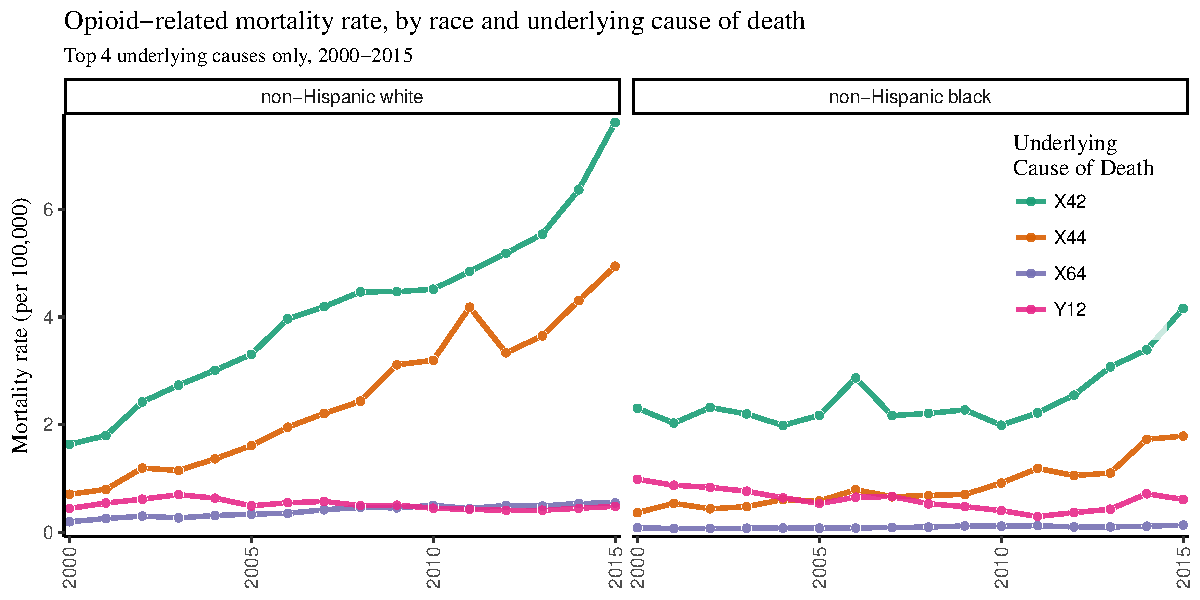
\includegraphics[width=1\textwidth]{./plots/paper_fig3_ucod_adjusted.pdf} 
 \caption{Underlying cause of death of opioid deaths by race, 2000--2015. The four largest categories have been highlighted: X42 (accidental drug overdose due to narcotics and psychodysleptics); X44 (accidental drug overdose due to unspecified drugs); Y12 (drug overdose due to narcotics and psychodysleptics with intent unclear); and X64 (suicide by drug overdose due to unspecified drugs). 
}
 \label{fig:code_race}
\end{figure}

\subsection{Opioid death rates by type of drug}

Figure \ref{fig:opioid_race} shows overall death rates by opioid type (T-code) and race. Note that some deaths may list more than one opioid code, in which case they are counted in the numerator of both opioid types. As such, the sum of these death rates may be more than the overall death rate illustrated in Figure \ref{fig:overall}. For both races the death rate due to heroin (T401) has risen over the past fifteen years --- and especially since 2010 --- to become the largest contributor to opioid-related deaths. 

The trend in death rates due to other natural and semi-synthetic opioids (T402) has been increasing for both the black and white populations, although it is a more important factor for the white population. The increase in this category of opioid has largely been caused by the increase in prescriptions and, consequently, overdoses, of hydrocodone and oxycodone, under the brand names Vicodin and OxyContin (Kolodny et al.\ 2015). Both painkillers are addictive, and have intense withdrawal symptoms. For many reasons prescription rates of such opioid painkillers are lower for the black population compared to the white population (e.g.,\ see Meghani et al.\ 2012). As such, black death rates due to opioids in T402 are lower. In 2010 OxyContin was reformulated to be less easily abused, making it harder to crush (and therefore be snorted or dissolved and injected). This reformulation may explain some of the leveling-off in the white death rate since 2010. 

The death rate due to methadone (T403) increased steadily through the early 2000s, especially for the white population. However, since around 2006 deaths due to methadone have decreased. This coincides with efforts by the Food and Drug Administration (FDA), Drug Enforcement Agency (DEA) and methadone manufacturers to issue warnings about the risks of prescribing methadone for pain and to limit prescription supply (Jones et al.\ 2016).

The other notable trend from Figure \ref{fig:opioid_race} is the sharp increase for both races in the T404 group, that is, synthetic opioids other than methadone. The rate of increase is similar to that of heroin, although it starts two or three years later. Most this increase is due to fentanyl and fentanyl compounds. Pharmaceutical fentanyl is a synthetic painkiller that is 50--100 times more powerful than morphine and is used for treating severe pain, typically advanced cancer pain. However, the presence of illicitly-made fentanyl in the form of acetyl- and furanyl-fentanyl has increased in recent years (CDC 2016a). These products are often mixed with heroin or cocaine to increase potency, and this can be done without the user's knowledge. The spike in 2006 in the T404 group, which is especially large for the black population, was also related to illicitly-produced fentanyl. However, the death rate declined after a large-scale operation by the DEA in 2006 that closed several fentanyl production facilities (CDC 2008).

The DEA notes that the true number of deaths due to fentanyl is likely to be even higher as ``many coroners' offices and state crime laboratories do not test for fentanyl or its analogs unless given a specific reason to do so'' (DEA 2015). The symptoms of fentanyl-related cases may be attributed to heroin because patients would present as if experiencing a heroin overdose and respond similarly to naloxone, albeit possibly requiring a larger dose (Stogner 2014). It is likely that much of the recent fentanyl increase is directly related to the heroin death rate increase. This is investigated further in Section \ref{section:multiple_cause}.

\begin{figure}[h!]
 \centering
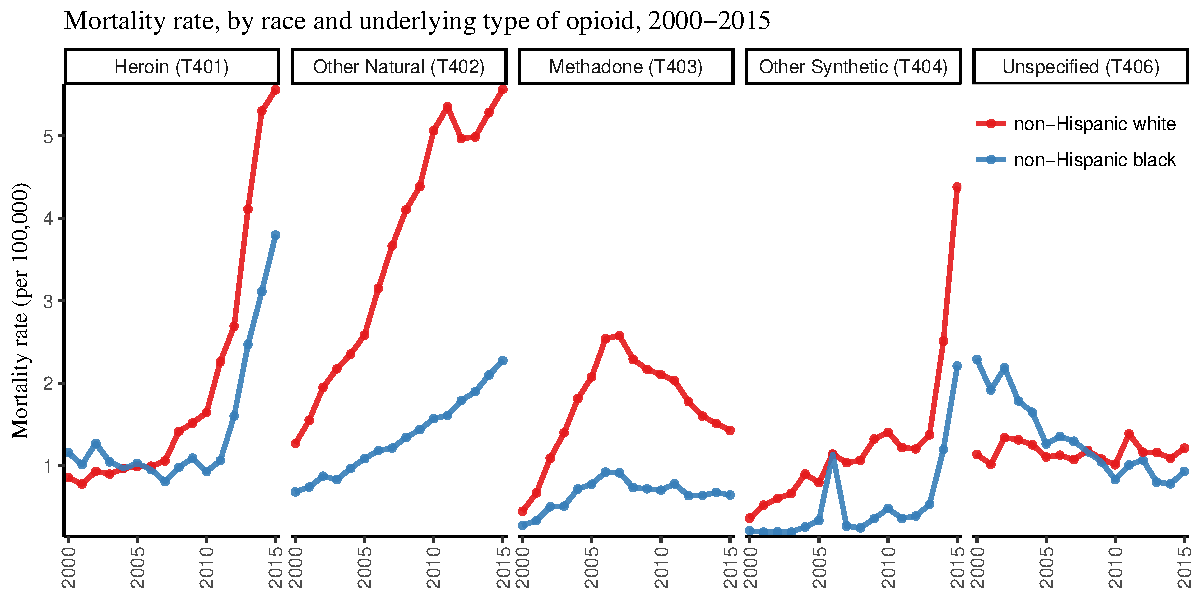
\includegraphics[width=0.95\textwidth]{./plots/paper_fig4_t40_adjusted_race_lines.pdf} 
 \caption{Death rates by underlying type of opioid and race, 2000--2015}
 \label{fig:opioid_race}
\end{figure}

In summary, the increase in opioid-related mortality has been largely due to accidental overdoses of opioids or a mixture of opioids and other drugs. The increase in the 2000--2010 period was more substantial for the white population and was due to prescription painkillers (Vicodin, OxyContin and methadone). Since 2010, the rates of opioid-mortality increase for both the white and black populations have been largely due to heroin and fentanyl. 

The key point from Figure \ref{fig:opioid_race} is that the gap in black-white opioid mortality rates seen in Figure \ref{fig:overall} was largely driven by the different mortality rates due to the prescription painkillers in the early 2000s. In contrast, the rate of increase in the more recent phenomena --- heroin and fentanyl --- has been similar for the black and white populations, and the gap in death rates is also smaller in an absolute sense. 

%%%%%%%%%%%%%%%%%%%
\section{Age patterns in opioid mortality} \label{section:age}
%In Section \ref{section:overall}, it was shown that there are distinct differences by race in the types of opioids underlying deaths. 
The types of opioids responsible for deaths are likely to vary with age, given some are illicit drugs, while others are prescription painkillers. Given the differences in the overall opioid-related death rates by race, patterns across age for the white and black population could be similar, but just lower for the black population. Alternatively, age patterns could be different. This section presents an analysis of opioid-related deaths by age group to determine age patterns across race and time. 

\subsection{Overall death rates by age}

Opioid-related mortality rates have increased for both populations in all age groups (Figures \ref{fig:asmr_curves} and \ref{fig:asmr_time}). However, the age profile is different across the two populations --- for the white population it is younger, and has become increasingly so over time (Figure \ref{fig:asmr_curves}). In 2015 the opioid death rate for the white population peaks in the 30-39 age group, whereas it peaks in the 50-59 age group for the black population. 

The two trends seen in the overall death rates (Figure \ref{fig:overall}) between 2000--2010 and 2010--2015 are observed in most age groups, but not all. Figure \ref{fig:asmr_time} shows that the increasing gap in opioid-mortality rates over the period 2000--2010 was driven by increases in age groups 20-49 in the white population. However, since 2010  the rate of increase in opioid mortality is similar in these age groups (even though the level is lower for the black population). Older age groups (50+) show similar death rates for both populations. %The average age at death due to opioid-related mortality is for whites in 2015 was 42 years, compared to 46 years for the black population. 

The gap in the opioid mortality rate across race is particularly large in the younger age groups (ages 20-39). In 2015 the white opioid mortality rate was as much as 3.6 times higher than the black opioid mortality rate (for the 20-29 age group). The effect of higher mortality rates is amplified by the lower overall mortality for the white population compared to the black population. For example, in 2015, opioid-related deaths accounted for over 20 per cent of all white deaths in the 20-29 age group, over four times higher than the peak in the black population, at around 5 per cent. This means that, not only are mortality rates higher for most age groups in the white population, opioid-related deaths also have a larger effect on overall mortality. Hypothetically, if all opioid-related deaths were removed, the overall life expectancy at age 15 for the white population would increase by 0.35 years. On the other hand, removing opioid deaths in the black population only increases life expectancy at age 15 by 0.16 years. In addition, even if the opioid deaths in the black population are removed at the level implied by the white opioid mortality rates, the increase in life expectancy at age 15 is 0.19 years, which is still less than for the white population. This is because other mortality is higher for the black population and so opioid deaths have a disproportionately smaller effect.\footnote{We calculated cause-deleted associated single decrement life tables using 2012 life tables for the United States provided by NCHS (Arias et al.\ 2016) and the method described in Wachter (2014, chapter 8).} 

%
%\begin{figure}[h!]
%\begin{subfigure} [b]{1\textwidth} 
% \centering
%\includegraphics[width=0.8\textwidth]{./plots/9d_asmr_race_year.pdf} 
% \caption{Age-specific opioid-mortality rate curves by race, 2000--2015}
% \label{fig:asmr_curves}
% \end{subfigure} ~
% \begin{subfigure} [b]{1\textwidth} 
% \centering
%\includegraphics[width=0.8\textwidth]{./plots/2b_age_spec_by_race.pdf} 
% \caption{Age-specific opioid-mortality rate over time, black, 2000--2015}
% \label{fig:asmr_time}
% \end{subfigure} ~
%\end{figure}

\begin{figure}[h!]
 \centering
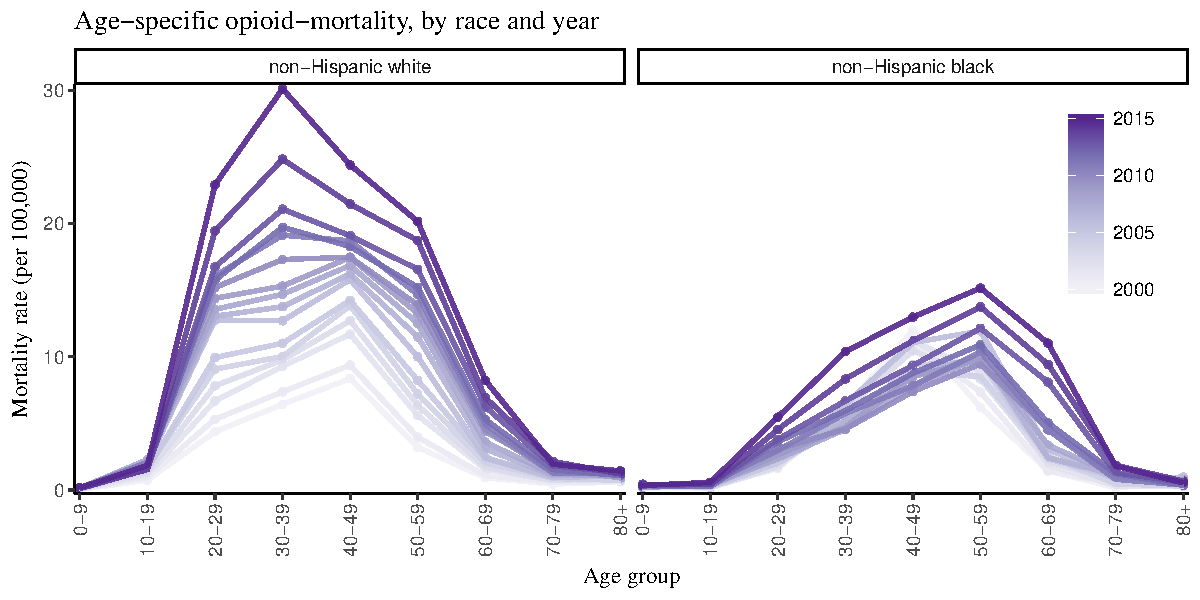
\includegraphics[width=0.95\textwidth]{./plots/paper_fig5_asmr_race_all.pdf} 
 \caption{Age-specific opioid-mortality rate curves by race, 2000--2015}
 \label{fig:asmr_curves}
\end{figure}

\begin{figure}[h!]
 \centering
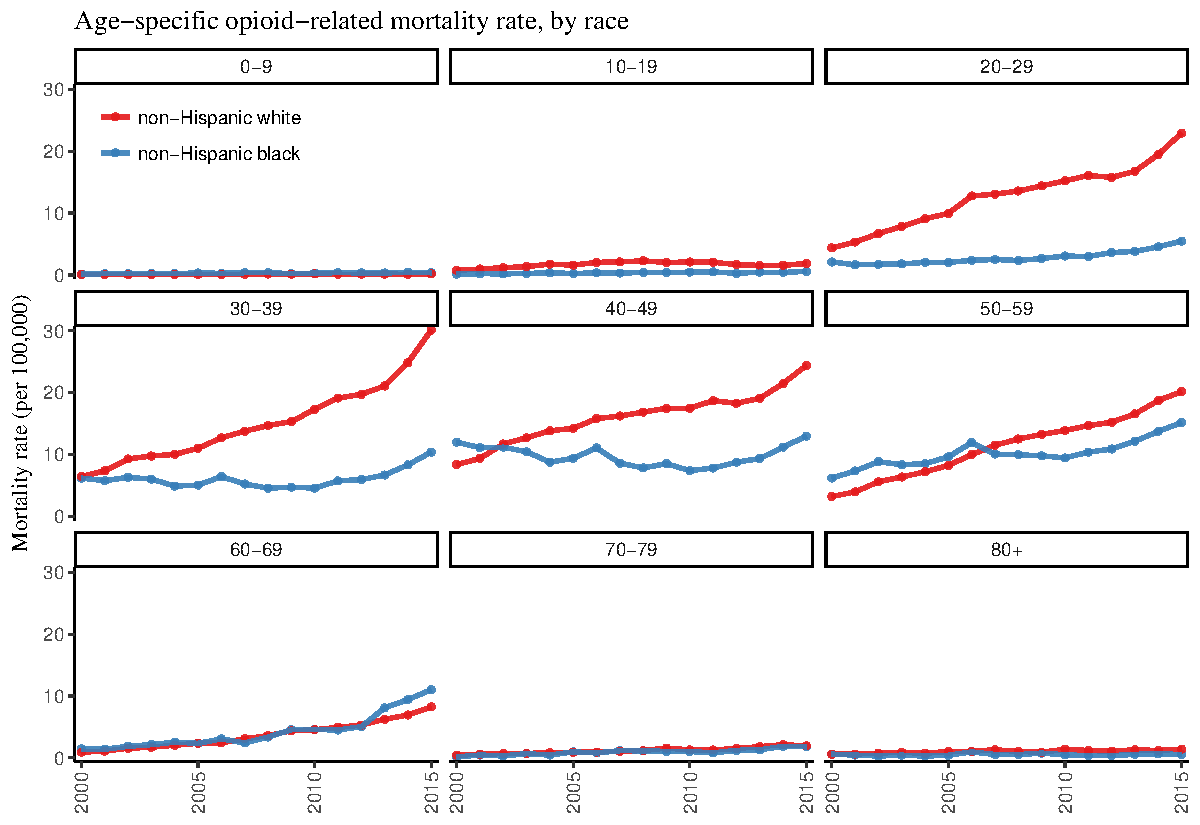
\includegraphics[width=0.95\textwidth]{./plots/paper_fig6_age_spec_by_race.pdf} 
 \caption{Age-specific opioid-mortality rate over time, 2000--2015}
 \label{fig:asmr_time}
\end{figure}

%\begin{figure}[h!]
% \centering
%\includegraphics[width=0.6\textwidth]{./plots/MA_asmr_prop.pdf} 
% \caption{Proportion of age-specific mortality that is related to opioids, 2015}
% \label{fig:asmr_prop}
%\end{figure}

%%%%%%%%%%%%%%%%%%%%%%%%

\subsection{Opioid types by age}
%\todo[inline, color = blue!40]{what is going on with unspecified opioids for blacks in earlier years. do they look like oxy deaths}
%\todo[inline, color = green!40]{Figure \ref{fig:tcode_race} get rid of opium; switch colors to rows}
%\todo[inline, color = green!40]{Figure \ref{fig:tcode_race_black} and white version: do as 10 year age groups}
%\todo[inline, color = green!40]{could be nice to combine 7a into relative risk}

Figure \ref{fig:tcode_race} further disaggregates age patterns by type of opioid. The patterns by opioid type observed in Figure \ref{fig:opioid_race} are generally replicated across all age groups; that is, the sharp increase in heroin and fentanyl since 2010; the gradual increase of other natural opioids (T402), in particular for the white population; and the decline of methadone since 2006. However, there are notable differences by race in the relative importance of the age groups. 

For the white population, the relative importance of natural and semi-synthetic opioids in the T402 category (mostly OxyContin and Vicodin) is high for all age groups, but increases with age. In addition, the sharp increases in heroin and fentanyl (T404) are also present in all age groups, but the relative importance of this pattern in terms of influencing age-specific mortality decreases with age.

For the black population, as discussed, the level of the T402 category is much lower than for the white population. However, the pattern is similar in that the relative importance increases with age. There is a much higher proportion of unspecified opioids for the black population, especially in the early years of the period, which could be understating the number of deaths due to prescription painkillers in categories T402 and T403 in the earlier years. The sharp increases in heroin and fentanyl (T404) are also present in all age groups, however, the relative importance of heroin and fentanyl increases with age in the black population. The opposite is true for the white population. This creates a cross-over in heroin death rates by race across age, which can be seen in the first row of Figure \ref{fig:tcode_race}.

In summary, although patterns in age-specific opioid-mortality rates by race show some similarities, there are also important differences. The age profile of white opioid deaths is much younger than for black opioid deaths, with peak mortality rates in 2015 being experienced by 30-39 year olds for the white population compared to 50-59 year olds for the black population. In addition, while the recent increase in heroin and fentanyl has generally been experienced by both races across all ages, the death rates due to this spike decrease by age for the white population, but increase with age for the black population. 
%
%\begin{figure}[h!]
%\begin{subfigure} [b]{1\textwidth} 
% \centering
%\includegraphics[width=0.95\textwidth]{./plots/7d_t40code_age_white.pdf} 
% \caption{Age-specific mortality rate by opioid type, white, 2000--2015}
% \label{fig:tcode_race_white}
% \end{subfigure} ~
% \begin{subfigure} [b]{1\textwidth} 
% \centering
%\includegraphics[width=0.95\textwidth]{./plots/7e_t40code_age_black.pdf} 
% \caption{Age-specific mortality rate by opioid type, black, 2000--2015}
% \label{fig:tcode_race_black}
% \end{subfigure} ~
%\end{figure}

\begin{figure}[h!]
 \centering
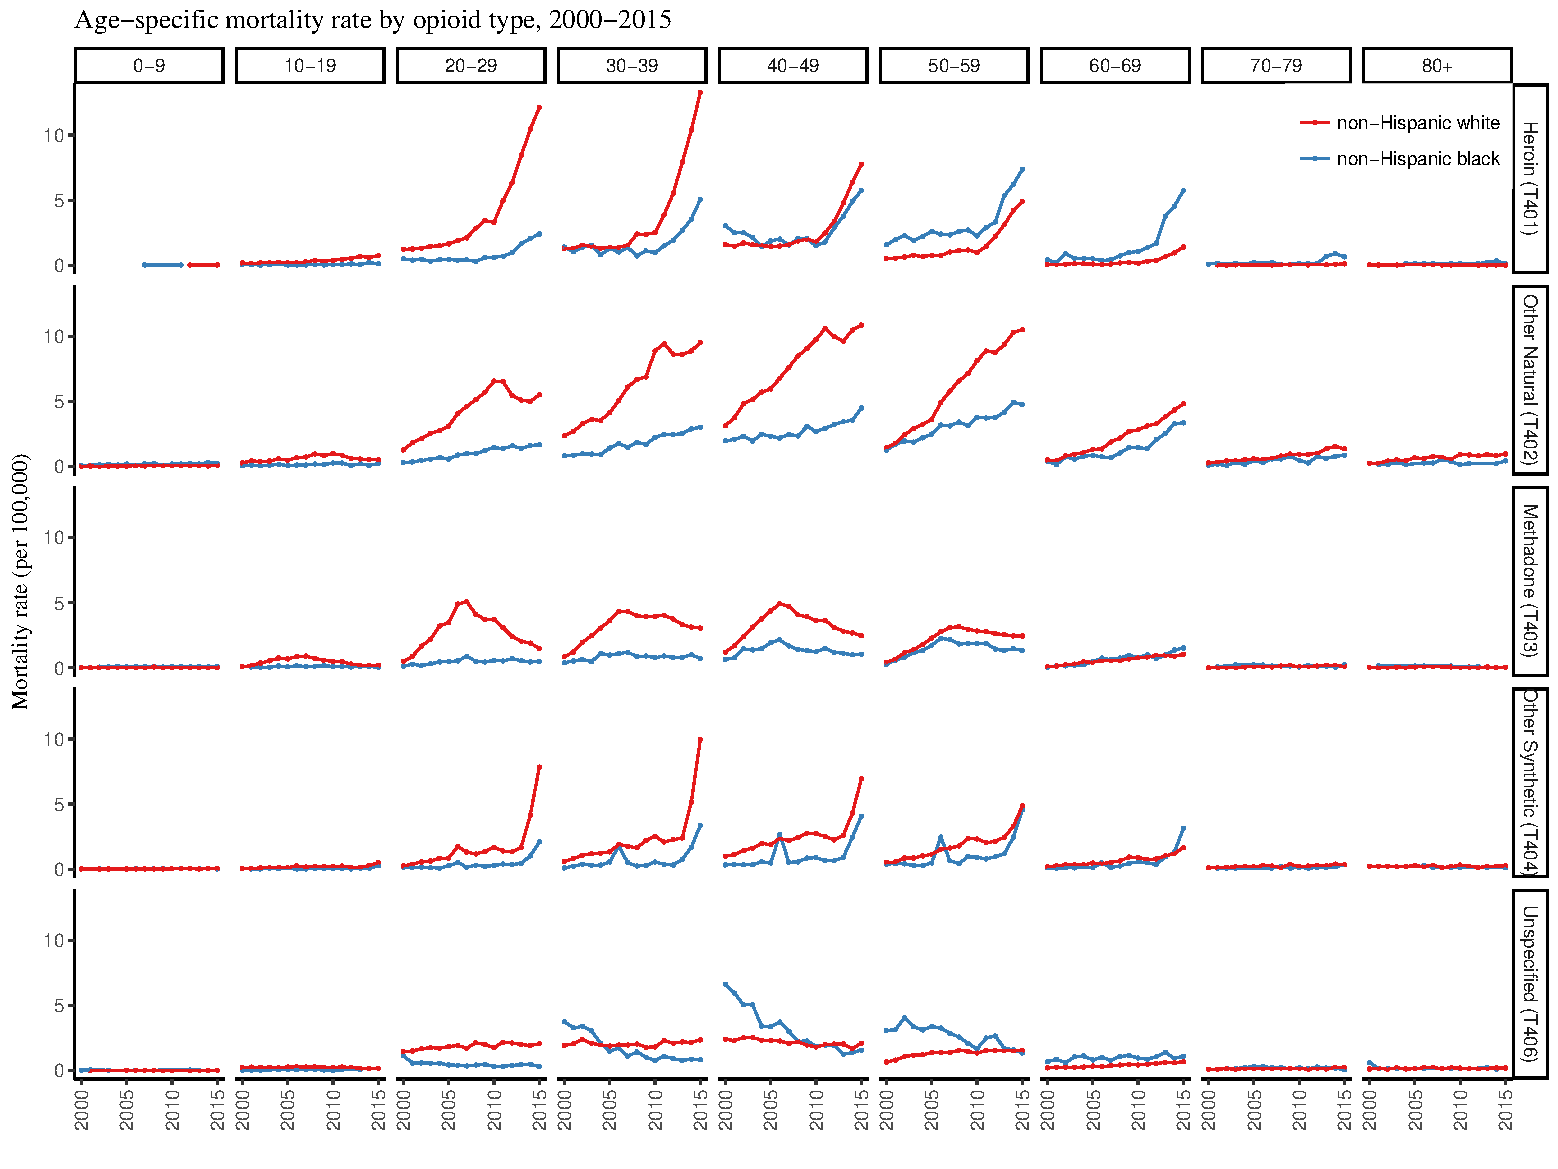
\includegraphics[width=1\textwidth]{./plots/paper_fig7_t40_notpretty.pdf} 
 \caption{Age-specific mortality rate by opioid type, 2000--2015}
 \label{fig:tcode_race}
\end{figure}


%%%%%%%%%%%%
\section{Multiple causes related to opioid deaths} \label{section:multiple_cause}
In previous sections, we observed that the change in the trend of opioid deaths that started around 2010 was largely due to substantial increases in the rate of heroin-related deaths, as well as fentanyl-related opioids since 2013. Given the similar and considerable rate of increase in the two drugs, one may expect that a large part of the increasing death rate is due to deaths from the drugs together, rather than separately. 

We can test this by looking at the multiple cause-of-deaths associated with opioid deaths. For opioid deaths, there is an underlying cause and up to 20 other contributing causes of death and at least one of those causes will be an opioid T-codes. The remaining contributing causes may include other drugs (opioid or non-opioid), or other existing health issues such as diabetes, heart disease, or mental and behavioral disorders. We focus on assessing changes in the co-presence of different drugs. 

%\subsection{Deaths in the presence of multiple opioids}
Many opioid deaths involve one opioid only. However, the number of deaths involving more than one opioid has increased (Figure \ref{fig:twomore}). In 2015, 22 per cent of white opioid deaths involved two or more types of opioids. Although the percentage for the black population was lower at the beginning of the period, by 2015 it had surpassed that of the white population, at 26 per cent. The proportion of deaths involving multiple opioids has increased since 2000 but the rate accelerated in 2013, in line with the increase in fentanyl-related deaths. The same pattern is not observed in the number of non-opioids per opioid death. 

\begin{figure}[h!]
 \centering
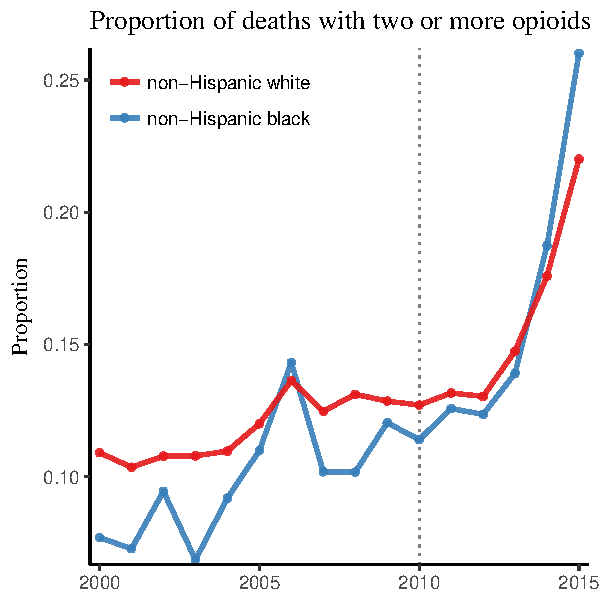
\includegraphics[width=0.5\textwidth]{./plots/paper_fig8_prop_2_more_v.pdf} 
 \caption{Proportion of opioid deaths that involve two or more opioids, 2000--2015}
 \label{fig:twomore}
\end{figure}

Focusing on heroin-related deaths, we find that the percentage of deaths that involve only heroin (and no other opioids) decreased by more than 15 percentage points for both races over the period 2013--2015. Deaths related to all major types of opioids have been associated with an increased presence of heroin since 2010 (Figure \ref{fig:401}). The proportion of deaths due to T402 opioids (mostly OxyContin and Vicodin) that also involve heroin has increased from around 0.5 per cent to 8 per cent for both races over the period 2010--2015. In addition, the proportion of methadone deaths (T403) that involve heroin has also increased. Therefore, an increasing number of heroin overdoses involve people who have also taken prescription opioid painkillers. This may suggest those who have become dependent on opioid painkillers are transitioning to heroin as prescriptions are restricted (Alpert et al.\ 2017).

The proportion of T404 opioid deaths that also involve heroin have increased at least ten-fold in the past few years, from around 2 per cent in 2012 to over 20 per cent in 2015. This dramatic increase corresponds to similar increases seen independently for heroin and fentanyl-type opioids (see Figure \ref{fig:opioid_race}), suggesting that much of the increase in both categories is due to deaths that involve both drug types. This implies that much of the increase in fentanyl opioid deaths is due to illegally manufactured fentanyl that is taken with heroin.  

It is not only opioids that are present in heroin-related deaths; often contributory causes of death include a mixture of opioids, other drugs and toxic substances. The most commonly occurring non-opioid toxic substances contributing to heroin deaths are cocaine, alcohol and Benzodiazepines (see Figure in Appendix \ref{tetris}). 

In summary, the proportion of opioid deaths that involve a mixture of opioids is increasing. This suggests that opioid deaths rates, in particular due to heroin, are increasing not only because of increased use, but potentially because of a change in use. In all cases of other-opioid deaths involving heroin, the proportion in the black population is slightly higher than for the white population, pointing to different drug-use behaviors. 

\begin{figure}[h!]
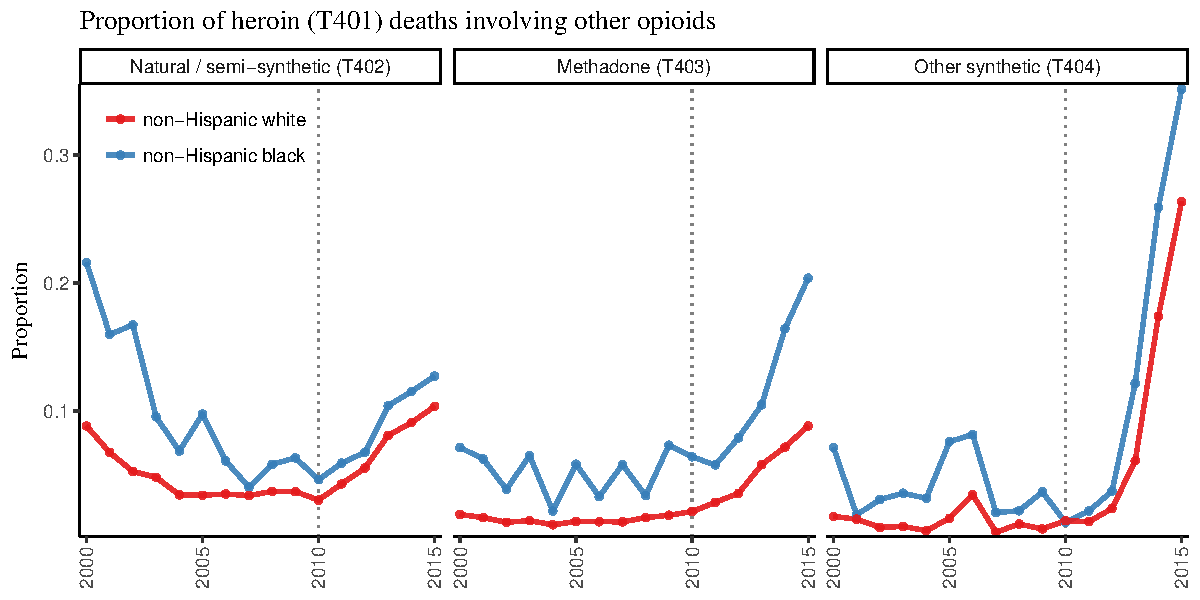
\includegraphics[width=0.95\textwidth]{./plots/paper_fig9_t401_combos_v.pdf} 
 \caption{Proportion of T402 (other natural and semi-synthetics), T403 (Methadone) and T404 (other synthetics) that also involve heroin}
 \label{fig:401}
\end{figure}


%\subsection{Contributory causes to opioid deaths}
%We analyzed contributory causes in opioid-related deaths over 2000--2015 to see which causes that are not drug poisoning related commonly occur in conjunction with opioid deaths. For each year, race and opioid T-code, we looked at the proportion of all deaths that included each contributory cause. 
%
%Each chart in Figures \ref{fig:matrix_1} and \ref{fig:matrix_2} represents a different opioid type (T401 - T404).\todo{link to high resolution of these charts?} For each chart, the x-axis is the year, and the y-axis is the code of the contributory cause. The color of each rectangle represents the proportion (on the log scale) of deaths for that year that list that particular code as a contributory cause. These charts are hard to read, as there are hundreds of different causes associated with the deaths from each of the opioid types. However, this `birds eye view' does illustrate several characteristics of the contributory causes underlying opioid deaths. Firstly, there is generally more heterogeneity in the underlying categories for whites, especially in the past few years. For example, for heroin deaths, in 2015 deaths in the black population had XX different contributory causes, compared to XX in the white population. \todo{calculate ave number of different contributory causes by race} This is likely just a function of the number of deaths -- there are many more white opioid deaths, so much chance of different types of underlying causes. 
%
%Secondly, there are clear `blocks' of underlying code types that occur in most years for both races. \todo{make charts of different blocks} We plot each of these blocks separately to ore easily discern patterns by race. 
%




%%%%%%%%%%%%%%%%
\section{Discussion}
%\todo[inline, color = blue!40]{Any overall data on increase in prescriptions}
%\todo[inline, color = blue!40]{Any overall data on heroin price}
In this paper we investigated trends in opioid-related deaths in the United States over the period 2000--2015 using multiple cause-of-death data. We focused on race-specific differences across age and in underlying drug types. 

The trend in opioid deaths since 2000 has two stages. The first, during 2000--2010, exhibited a steady increase in the opioid death rate for the white population, while opioid-related mortality for the black population remained fairly constant. The increase over this period was mostly due to prescription opioids, namely OxyContin, Vicodin and methadone. The second period, from 2010 onwards, exhibited a higher rate of increase in the opioid death rate, and increases were similar for both the white and black populations. Increases in this period have largely been driven by increases in deaths due to heroin and fentanyl-related opioids. We found evidence to suggest that increases in deaths due to heroin and fentanyl have occurred from deaths that involve a mixture of both drugs. Despite recent similar increases, opioid mortality rates for the white population remain higher, with the overall death rate being about double that of the black population. There are also notable differences across age groups between the two races, with the white population exhibiting a comparatively younger age profile. There are several questions raised by this analysis. We do not attempt to answer them all here but rather present a discussion of the issues to motivate future research. 

Firstly, why has the death rate due to heroin and fentanyl-related drugs increased so rapidly since 2010? Previous research has found strong evidence to suggest that much of the increase in heroin overdoses is due a substitution effect since the reformulation of OxyContin. Alpert et al.\ (2017) exploited state-wide variation in reformulations to show this shift may have caused as much as 80 per cent of the three-fold increase in heroin mortality since 2010. While the supply of prescription opioids is increasingly restricted --- through the reformulation of OxyContin into an abuse deterrent form, as well as the introduction of national and state run restriction programs (for example, Prescription Drug Monitoring Programs and the Medicaid Lock-In Program) --- the supply of heroin in the United States continues to increase, and prices continue to fall (ONDCP, 2015). The increased mortality rate due to heroin is likely to be partly due to increased exposure to risk, given the likely increase in the number of people using heroin. However, the increased presence of more fatal forms of heroin mixed with fentanyl-type compounds are also likely to be increasing the mortality rate. Decomposing the increase in heroin deaths to determine how much is due to increased use compared with increased availability of more potent forms could have different implications for the types of health policies employed to reduce heroin addiction and eventual overdoses. Given a likely difference in price and distribution network location, we may expect differences in the competing effects by race, rurality and socioeconomic status. A more detailed version of the multiple cause-death data file (which indicates place of residence) combined with survey data on drug use (for example, the National Survey on Drug Use and Health (NSDUH)) would help to investigate this issue. 

Secondly, there are several questions regarding differences by race. The substantial gap in the white-black opioid mortality rate that developed during the 2000--2010 period was largely driven by differential use of prescription opioids across the two races. Previous research has documented this phenomena across a wide range of years, socioeconomic and age groups, and medical settings (e.g.,\ see Chen et al.\ 2005; McCabe et al.\ 2005; Kelly et al.\ 2008; Meghani et al.\ 2012; and Singhal et al.\ 2016). It is then important to examine why the recent rates of increase in opioid deaths are similar for both the white and black populations, given the relative absence of past opioid-related deaths. The likely increased demand for heroin that has occurred through the restriction of prescription opioids has made heroin easier to obtain and more affordable (ONDCP, 2015). Given the evidence for a substitution effect in the white population, users of other, non-opioid drugs, in the black population should be investigated to see whether they are substituting that for heroin. Finally, further investigation is needed into why the age distribution of opioid deaths in the black population is older than of the white population. This could be for several reasons. The recent heroin epidemic has been largely focused in rural areas (Keyes et al.\ 2014). Thus, the differing age distribution across race could partly be a consequence of the demographic composition of the areas where exposure is highest. In addition, the overall demographics of heroin users has changed over the past few decades, with users switching from being predominately black to white (Cicero et al.\ 2014). Therefore the observation of higher opioid death rates at older ages for the black population could partially be a cohort effect. Further investigation of these issues could draw on different data sources, including a more detailed multiple cause-death data file, census data, data on drug use from NSDUH and data on drug seizures and arrests. 

In this paper, we highlighted several key characteristics of mortality due to opioids in the United States. The nature of the epidemic has changed over the past fifteen years, and had different impacts on the black and white populations. Importantly, there has been an increase in mortality due to opioids since 2010 for both races, and this trend shows no sign of slowing. A better understanding of the differences across race and how they relate to the use of other drugs, place of residence, and socioeconomic status, is necessary to improve health policy and rehabilitation programs across the country. 

%%%%%%%%%%%%%%%%%
\newpage
\appendix
\section{Contributory toxic substances underlying heroin deaths, 2000--2015} \label{tetris}
\begin{figure}[h!]
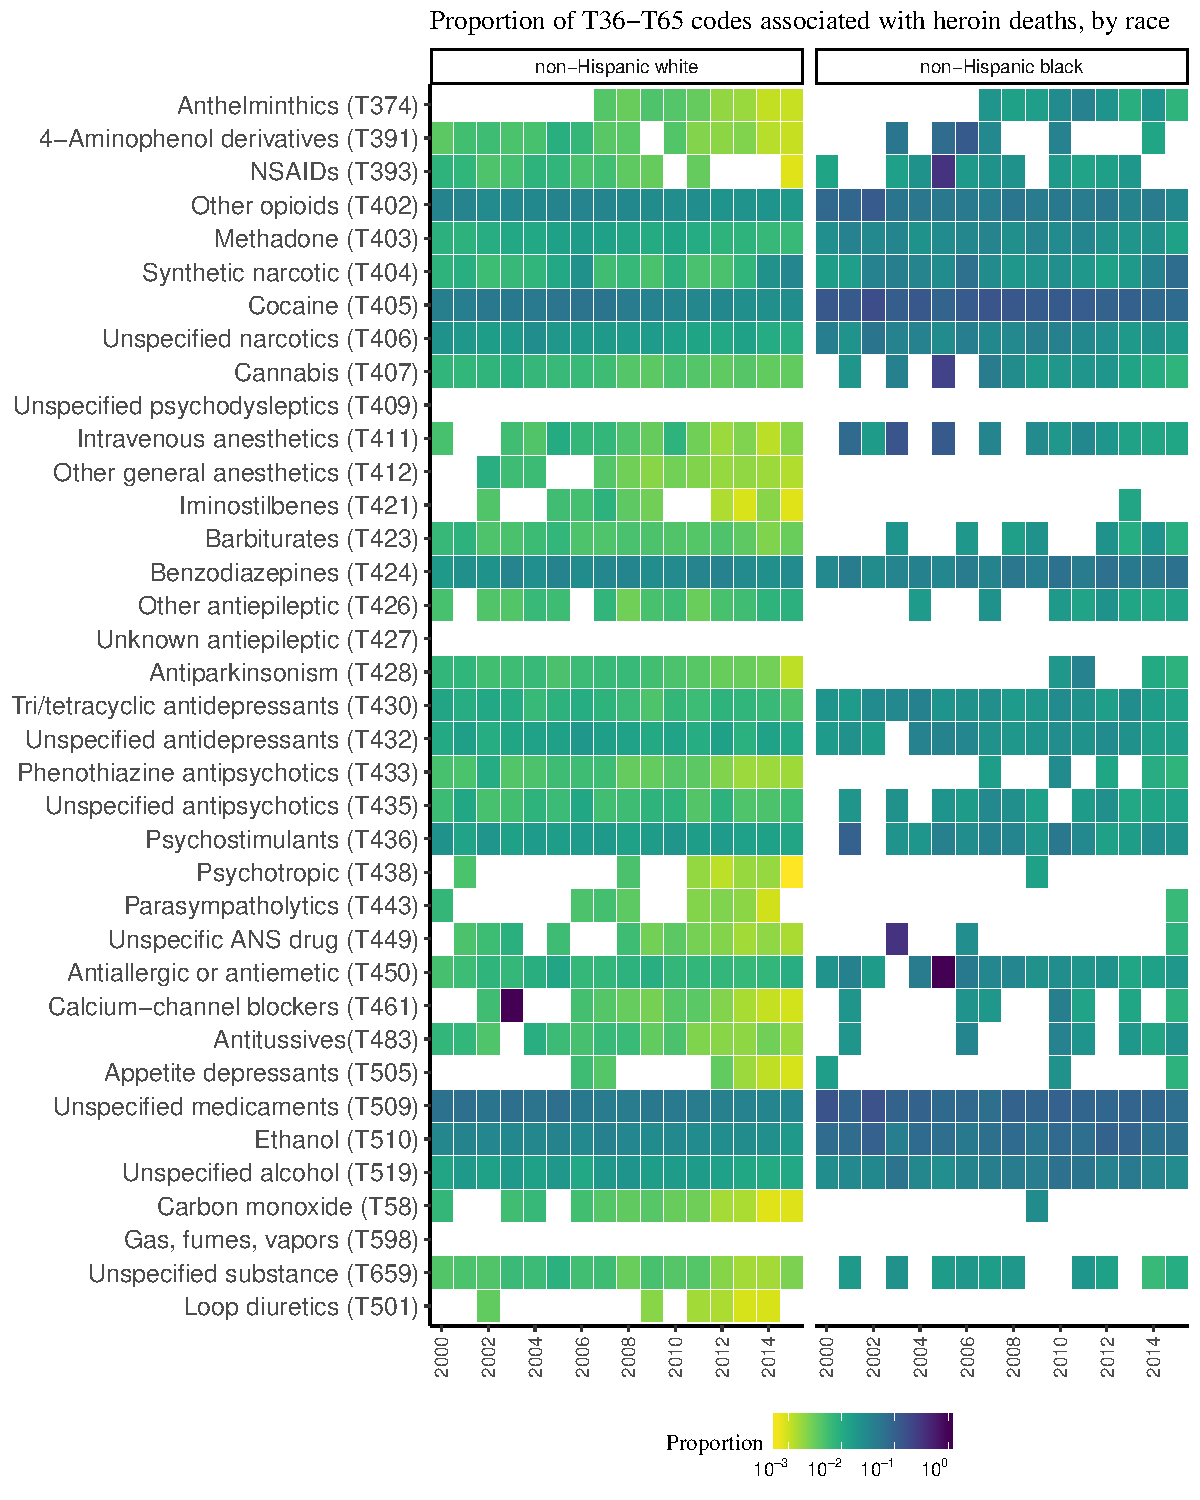
\includegraphics[width=0.95\textwidth]{./plots/t_code_plot.pdf} 
 \caption{Contributory toxic substances to heroin deaths, 2000--2015. Each colored square represents the proportion (plotted on log scale) of heroin deaths in that year/race that involved the substance listed on the y-axis. Only causes that had non-zero proportions for at least three consecutive years are shown. }
 \label{fig:401}
\end{figure}


%%%%%%%%%%%%%%%%%%%%%%%%%%%%%%
\newpage
\section*{References}
\begin{description}
\item Alpert A, Powell D and Pacula RL (2017); `Supply-Side Drug Policy in the Presence of Substitutes: Evidence from the Introduction of Abuse-Deterrent Opioids', \textit{RAND Working Paper}, WR-1181, January 2017. 
\item Arias E, Heron, M and Xu, J (2016): `United States Life Tables, 2012', \textit{National Vital Statistics Reports}, 65(8). \url{www.cdc.gov/nchs/data/nvsr/nvsr65/nvsr65_08.pdf}, accessed April 7 2017.
\item Case, A and Deaton, A (2017): `Mortality and morbidity in the 21st century', \textit{Brookings Papers on Economic Activity}, BPEA Conference Drafts, March 23--24, 2017. \\\url{www.brookings.edu/wp-content/uploads/2017/03/6_casedeaton.pdf}, accessed April 7 2017.
\item Centers for Disease Control and Protection (CDC) (2008): `Nonpharmaceutical Fentanyl-Related Deaths --- Multiple States, April 2005--March 2007', \textit{Morbidity and Mortality Weekly Report (MMWR)}, July 25 2008, Centers for Disease Control and Protection. \url{www.cdc.gov/mmwr/preview/mmwrhtml/mm5729a1.htm}, accessed April 7 2017.
\item Centers for Disease Control and Protection (CDC) (2016): `Reported Law Enforcement Encounters Testing Positive for Fentanyl Increase Across US'. \url{www.cdc.gov/drugoverdose/data/fentanyl-le-reports.html}, accessed April 7 2017.
\item Chen, I, Kurz, J, Pasanen, M, Faselis, C, Mukta P, Staton, L, O'Rorke, J, Menon, M, Genao, I, Wood, J, Mechaber, AJ, Rosenberg E, Carey T, Calleson, D and Cykert, S (2005): `Racial Differences in Opioid Use for Chronic Nonmalignant Pain', \textit{Journal of General Internal Medicine}, 20(7): 593--598.
\item Cicero TJ, Ellis, MS, Surratt, HL and Kurtz, SP (2014): `The Changing Face of Heroin Use in the United States: A Retrospective Analysis of the Past 50 Years', \textit{JAMA Psychiatry}, 71(7):821--826.
\item Dart, RC, Surratt, HL, Cicero, TJ, Parrino, MW, Severtson SG, Bucher-Bartelson, B and Green JL (2015): `Trends in Opioid Analgesic Abuse and Mortality in the United States', \textit{New England Journal of Medicine}, 372(3): 241--248.
\item Davis, GG, and the National Association of Medical Examiners and American College of Medical Toxicology Expert Panel on Evaluating
and Reporting Opioid Deaths (2014): `Complete Republication: National Association of Medical Examiners Position Paper: Recommendations for the Investigation, Diagnosis, and Certification of Deaths Related to Opioid Drugs', \textit{Journal of Medical Toxicology}, 10:100--106.
\item Drug Enforcement Agency (DEA) (2015): `National Heroin Threat Assessment Summary', \textit{DEA Intelligence Report}, DEA-DCT-DIR-039-15, April 2015. \\\url{www.dea.gov/divisions/hq/2015/hq052215_National_Heroin_Threat_Assessment_Summary.pdf}, accessed April 7 2017.
\item Frenk, SM, Porter, KS, Paulozzi, LJ (2015): `Prescription Opioid Analgesic Use Among Adults: United States, 1999--2012', \textit{NCHS Data Brief}, No. 189, February 2015. 
\item Jones, CM, Baldwin, FT, Manocchio, T, White, JO and Mack, KA (2016): `Trends in Methadone Distribution for Pain Treatment, Methadone Diversion, and Overdose Deaths ---United States, 2002--2014', \textit{Morbidity and Mortality Weekly Report (MMWR)}, July 8 2016, Centers for Disease Control and Protection. \url{www.cdc.gov/mmwr/volumes/65/wr/mm6526a2.htm}, accessed April 7 2017.
\item Kelly, JP, Cook, SF, Kaufman, DW, Anderson, T, Rosenberg, L and Mitchell, AA (2008): `Prevalence and characteristics of opioid use in the US adult population', \textit{Pain}, 138: 507--513.
\item Keyes, KM, Cerda, M, Brady, JE, Havens, JR and Galea, S (2014): `Understanding the Rural-Urban Differences in Nonmedical Prescription Opioid Use and Abuse in the United States', \textit{American Journal of Public Health}, 104(2):e52--e59.
\item Kolata, G and Cohen S (2016): `Drug Overdoses Propel Rise in Mortality Rates of Young Whites', \textit{New York Times}. \url{www.nytimes.com/2016/01/17/science/drug-overdoses-propel-rise-in-mortality-rates-of-young-whites.html},  accessed April 7 2017.
\item Kolodny, A, Courtwright, DT, Hwang, CS, Kreiner P, Eadie, JL, Clark TW, Alexander, GC (2015): `'The Prescription Opioid and Heroin Crisis: A Public Health Approach to an Epidemic of Addiction', \textit{Annual Review of Public Health}, 36:559--74.
\item Lane, C (2016): `The opioid epidemic: For whites only?', \textit{Washington Post}. \url{www.washingtonpost.com/blogs/post-partisan/wp/2016/08/18/the-opioid-epidemic-for-whites-only/},  accessed April 7 2017. 
\item McCabe, SE, Teter, CJ, Boyd, CJ, Knight, JR and Wechsler H (2005):`Nonmedical use of prescription opioids among U.S. college students: Prevalence and correlates from a national survey', \textit{Addictive Behaviors}, 30: 789--805.
\item Meghani, SH, Byun, E and Gallagher, RM (2012): `Time to Take Stock: A Meta-Analysis and Systematic Review of Analgesic Treatment Disparities for Pain in the United States', \textit{Pain Medicine}, 13: 150--174.
\item National Center for Health Statistics (NCHS) (2016): `Data Access - Vital Statistics Online (Mortality Multiple Cause Files)'. \url{www.cdc.gov/nchs/data_access/vitalstatsonline.htm}, accessed April 7 2017. 
\item Office of National Drug Control Policy (ONDCP) (2015):`National Drug Control Strategy: Data Supplement'. \url{obamawhitehouse.archives.gov/sites/default/files/ondcp/policy-and-research/2015_data_supplement_final.pdf}, accessed April 7 2017. 
\item Paulozzi, LJ, Budnitz, DS, Xi, Y (2006): `Increasing deaths from opioid analgesics in the United States', \textit{Pharmacoepidemiology and Drug Safety}, 15: 618--627. 
\item Rudd, RA, Aleshire, N, Zibbell, JE and Gladden, RM (2016): `Increases in Drug and Opioid Overdose Deaths: United States, 2000--2014', \textit{Morbidity and Mortality Weekly Report (MMWR)}, December 30, 2016. Centers for Disease Control and Protection. \url{www.cdc.gov/mmwr/volumes/65/wr/mm655051e1.htm}, accessed April 7 2017.
\item Singhal, A, Tien, Y and Hsia, RY (2016): `Racial-Ethnic Disparities in Opioid Prescriptions at Emergency Department Visits for Conditions Commonly Associated with Prescription Drug Abuse', \textit{PLOS One}, DOI:10.1371/journal.pone.0159224.
\item Wachter, KW (2014): \textit{Essential Demographic Methods}, Harvard University Press, Cambridge, MA, USA.  
\item White House (2016): `Fact Sheet: Obama Administration Announces Prescription Opioid and Heroin Epidemic Awareness Week'. \url{obamawhitehouse.archives.gov/the-press-office/2016/09/19/fact-sheet-obama-administration-announces-prescription-opioid-and-heroin}, accessed April 7 2017.
\item White House (2017): `President Donald J. Trump Signs an Executive Order Establishing the President's Commission on Combating Drug Addiction and the Opioid Crisis'. \url{https://www.whitehouse.gov/the-press-office/2017/03/30/president-donald-j-trump-signs-executive-order-establishing-presidents}, accessed April 7 2017.
\item World Health Organization (WHO) (2017): `List of Official ICD-10 Updates'. \url{www.who.int/classifications/icd/icd10updates/en/}, accessed April 7 2017.
\item World Health Organization (WHO) (2016): `ICD-10 Version:2016'. \url{apps.who.int/classifications/icd10/browse/2016/en}, accessed April 7 2017.
\end{description}





\end{document}

